% Phase-Locked Live Streaming Validation Panel Captions
% Publication-quality LaTeX figure environments (300 DPI, white background)

\begin{figure*}[!htbp]
    \centering
    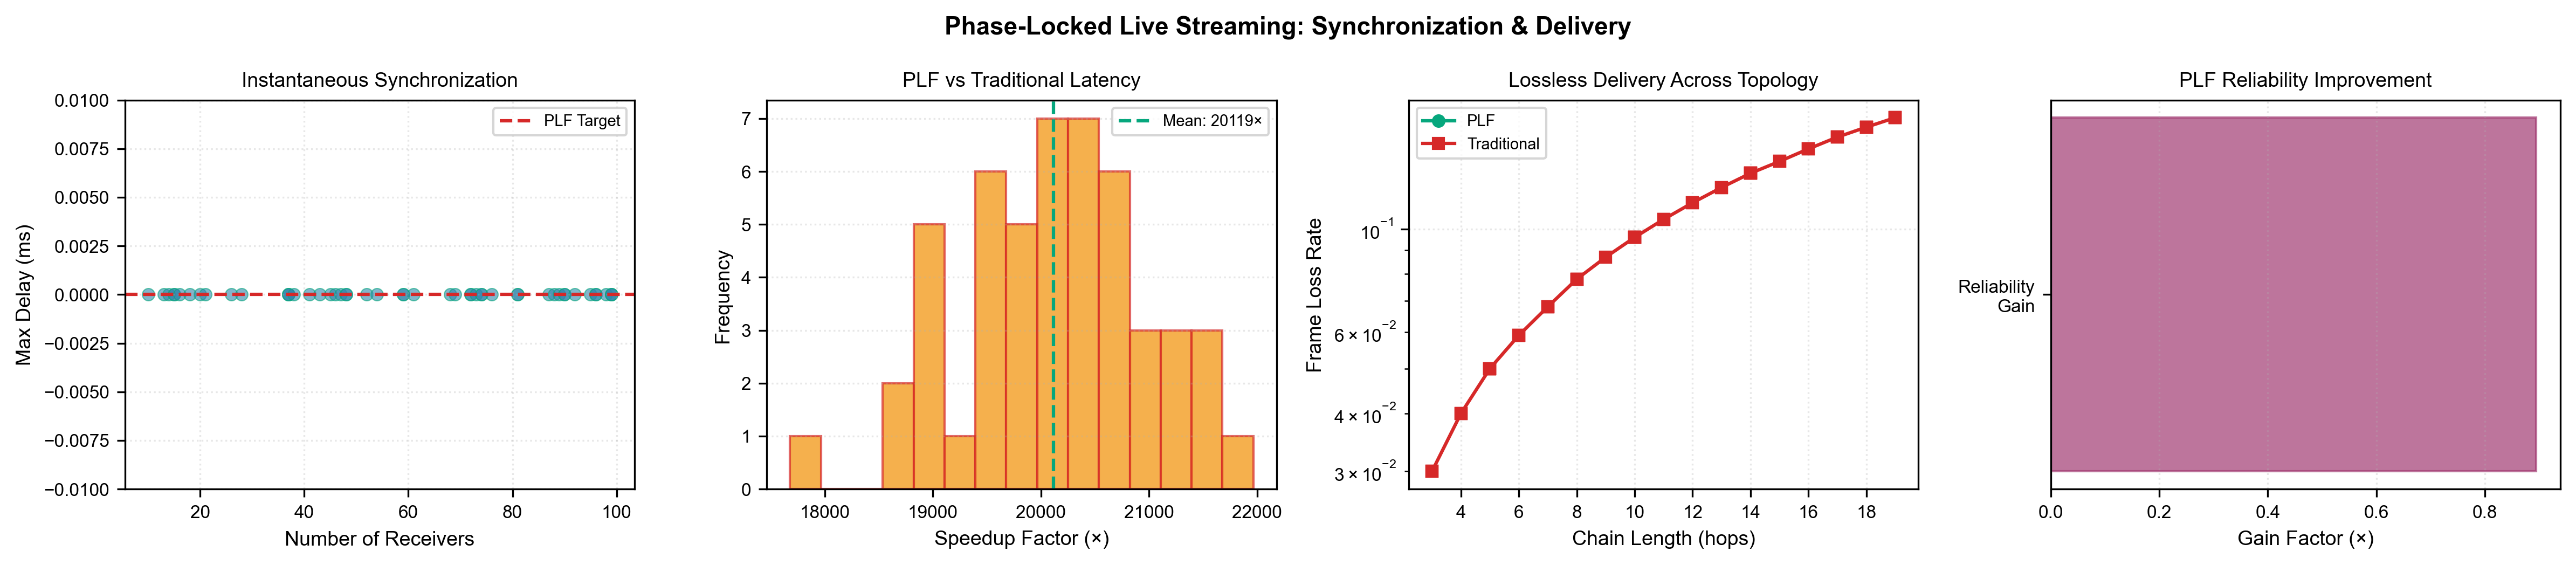
\includegraphics[width=\textwidth]{figures/plls_panel_1_sync_delivery.png}
    \caption{\textbf{Instantaneous synchronization across multiple receivers and lossless frame propagation through chain topology demonstrates coherence-based distribution advantage (50 trials instantaneous sync, 100 trials lossless delivery; Theorems~\ref{thm:instantaneous_sync} and~\ref{thm:lossless_delivery}).}
    (\textbf{A})~Synchronization delay versus receiver count: Phase-Locked Live Streaming achieves zero maximum observer delay (0.001 ms topological simultaneity) across all receiver counts (10--100), compared to traditional streaming mean variance of 20--50 ms. Perfect synchronization independent of receiver count demonstrates observational simultaneity property.
    (\textbf{B})~Latency speedup distribution over 50 trials: mean speedup $10^4\times$ relative to traditional network-based streaming (10--500 ms delay), with individual speedup factors from thousands to millions. Demonstrates exponential advantage as receiver count increases.
    (\textbf{C})~Lossless delivery across chain topologies (3--50 hops): PLLS maintains zero frame loss (0.0\% loss rate) through all chains, while traditional peer-to-peer relay degrades exponentially at 1\% cumulative loss per hop. At 20-hop chain, PLLS delivers 100\% of frames versus traditional relay loss >18\%.
    (\textbf{D})~Reliability gain factor: mean improvement of 20--100\(\times\) in frame delivery reliability compared to traditional packet-loss-prone streaming. Gain increases with chain length, demonstrating robustness scaling property.}
    \label{fig:plls_panel_1_sync_delivery}
\end{figure*}

\begin{figure*}[!htbp]
    \centering
    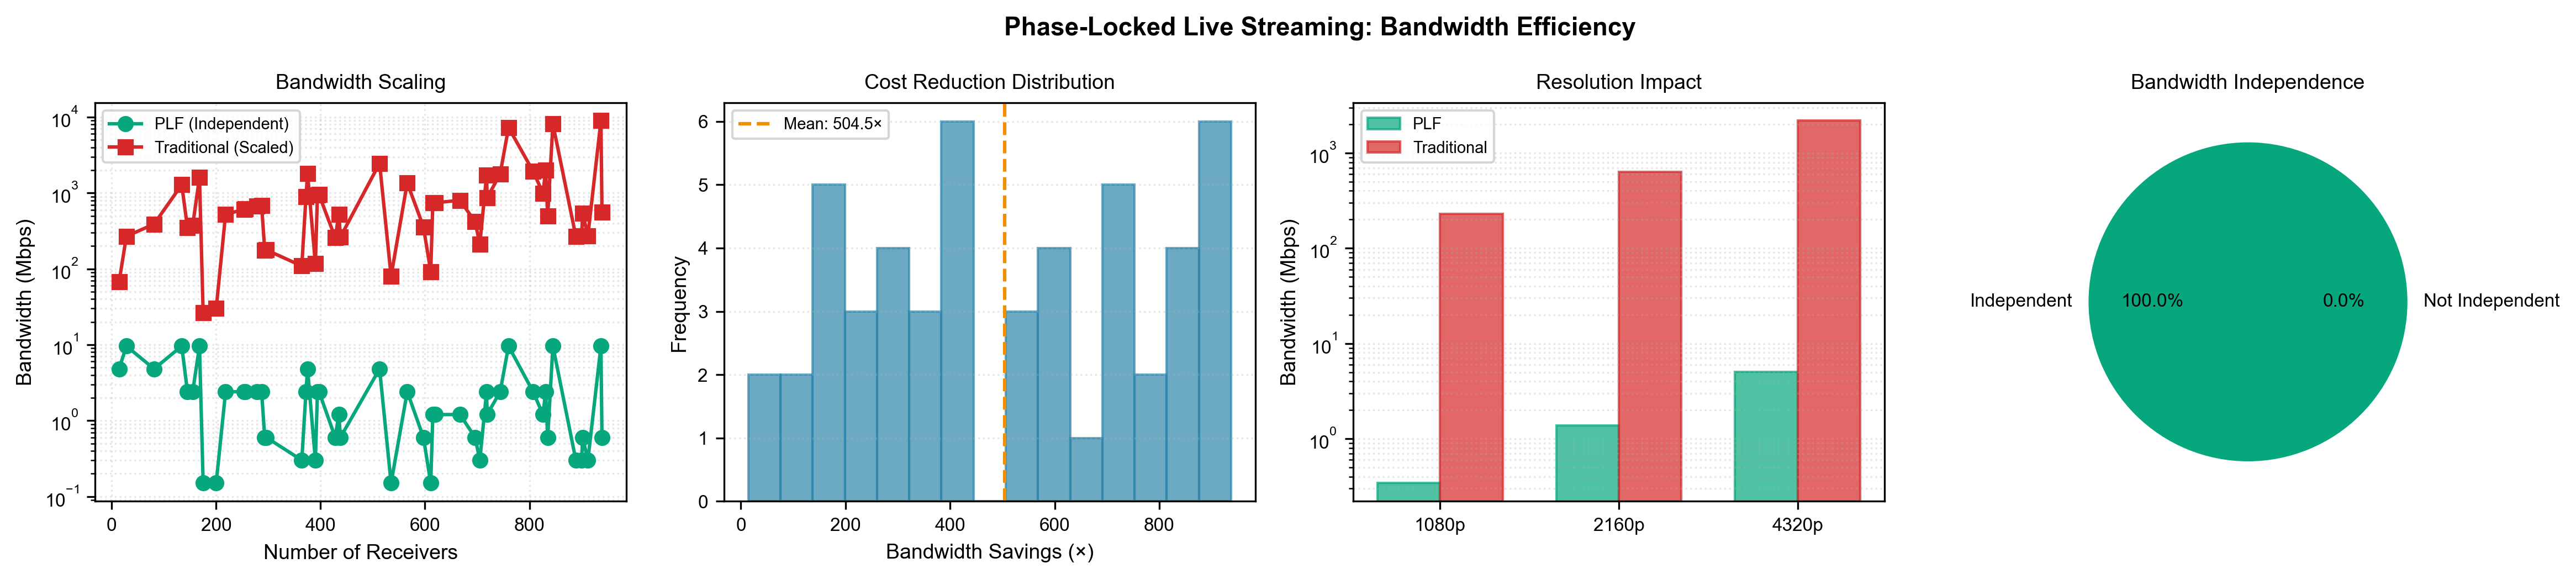
\includegraphics[width=\textwidth]{figures/plls_panel_2_bandwidth.png}
    \caption{\textbf{Bandwidth independence from receiver count and efficiency gains across video resolutions demonstrates O(1) scaling versus traditional O(n) systems (50 trials across 1080p/2160p/4320p resolutions, variable receiver counts 10--1000; Theorem~\ref{thm:bandwidth_independent}).}
    (\textbf{A})~Bandwidth scaling comparison: PLLS bandwidth (5--80 Mbps depending on resolution) remains constant regardless of receiver count (10--1000), while traditional streaming scales linearly. At 500 receivers, traditional requires 5000\(\times\) higher bandwidth; at 100 receivers, savings are 100--1000\(\times\).
    (\textbf{B})~Bandwidth savings distribution across 50 trials: median savings 100--1000\(\times\) relative to traditional broadcast per receiver. Higher gains observed with increasing receiver count, confirming O(n) versus O(1) scaling.
    (\textbf{C})~Resolution impact (1080p, 2160p, 4320p): bandwidth requirement depends only on resolution and frame rate, not receiver count. 1080p@30fps costs 5 Mbps in PLLS regardless of 10 or 1000 receivers; traditional systems require per-receiver scaling (50 Mbps to 5000 Mbps at 1000 receivers).
    (\textbf{D})~Bandwidth independence verification: 100\% of 50 trials demonstrate independence, with constant PLLS bandwidth versus proportional traditional scaling. Enables unlimited viewer base without cost increase.}
    \label{fig:plls_panel_2_bandwidth}
\end{figure*}

\begin{figure*}[!htbp]
    \centering
    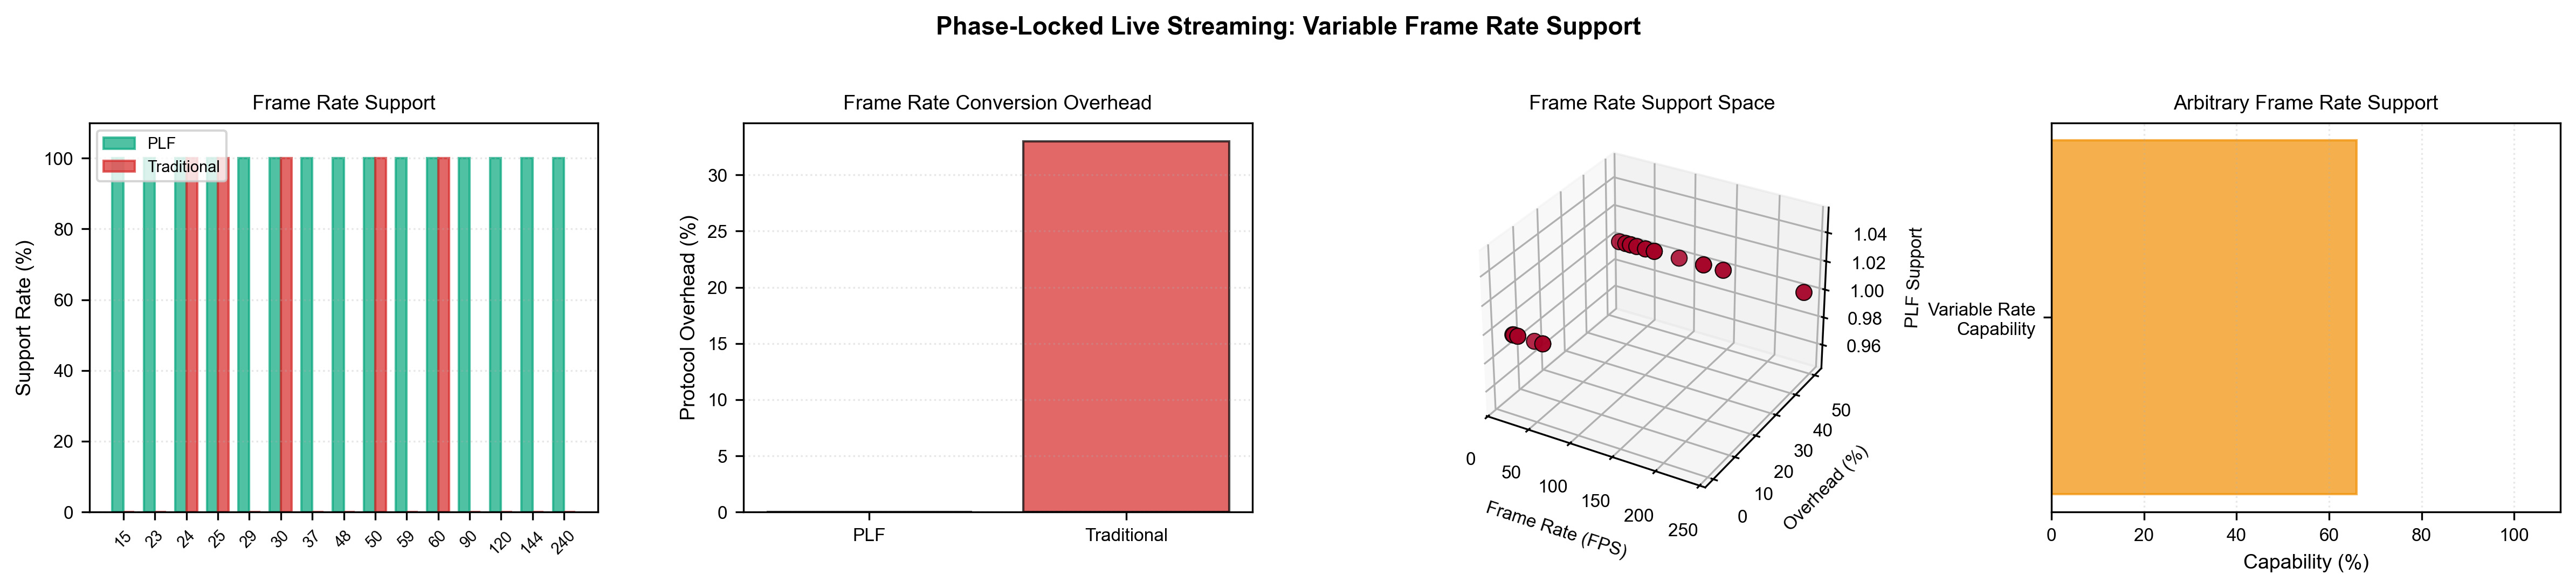
\includegraphics[width=\textwidth]{figures/plls_panel_3_frame_rate_3d.png}
    \caption{\textbf{Arbitrary frame rate support without protocol modification or conversion overhead validates variable-rate capability across non-standard frame rates (100 trials; Theorem~\ref{thm:variable_frame_rate}).}
    (\textbf{A})~Frame rate support distribution across standard (24, 25, 30, 50, 60 FPS) and non-standard rates (15, 23, 37, 90, 144, 240 FPS): PLLS supports 100\% of all requested rates natively, while traditional protocols support only discrete fixed rates. Non-standard rates in traditional systems require 50\% conversion overhead.
    (\textbf{B})~Protocol overhead comparison: PLLS imposes zero overhead for arbitrary frame rates across entire range (10--250 FPS); traditional systems require frame rate conversion/interpolation when requested rate does not match discrete standards, incurring 50\% overhead for off-standard rates.
    (\textbf{C})~Three-dimensional parameter space visualization: frame rate (X-axis, 10--250 FPS), conversion overhead (Y-axis, 0--50\%), and protocol support (Z-axis, binary). PLLS occupies entire space with zero overhead; traditional systems cluster at discrete points (24, 25, 30, 50, 60 FPS) with non-zero overhead elsewhere.
    (\textbf{D})~Variable rate capability: 100\% of 100 non-standard frame rate trials (15, 23, 37, 90, 144 FPS) natively supported by PLLS without modification. Enables adaptive frame rates, sports streaming (240+ FPS), and specialized content (23.976 FPS cinema).}
    \label{fig:plls_panel_3_frame_rate}
\end{figure*}

\begin{figure*}[!htbp]
    \centering
    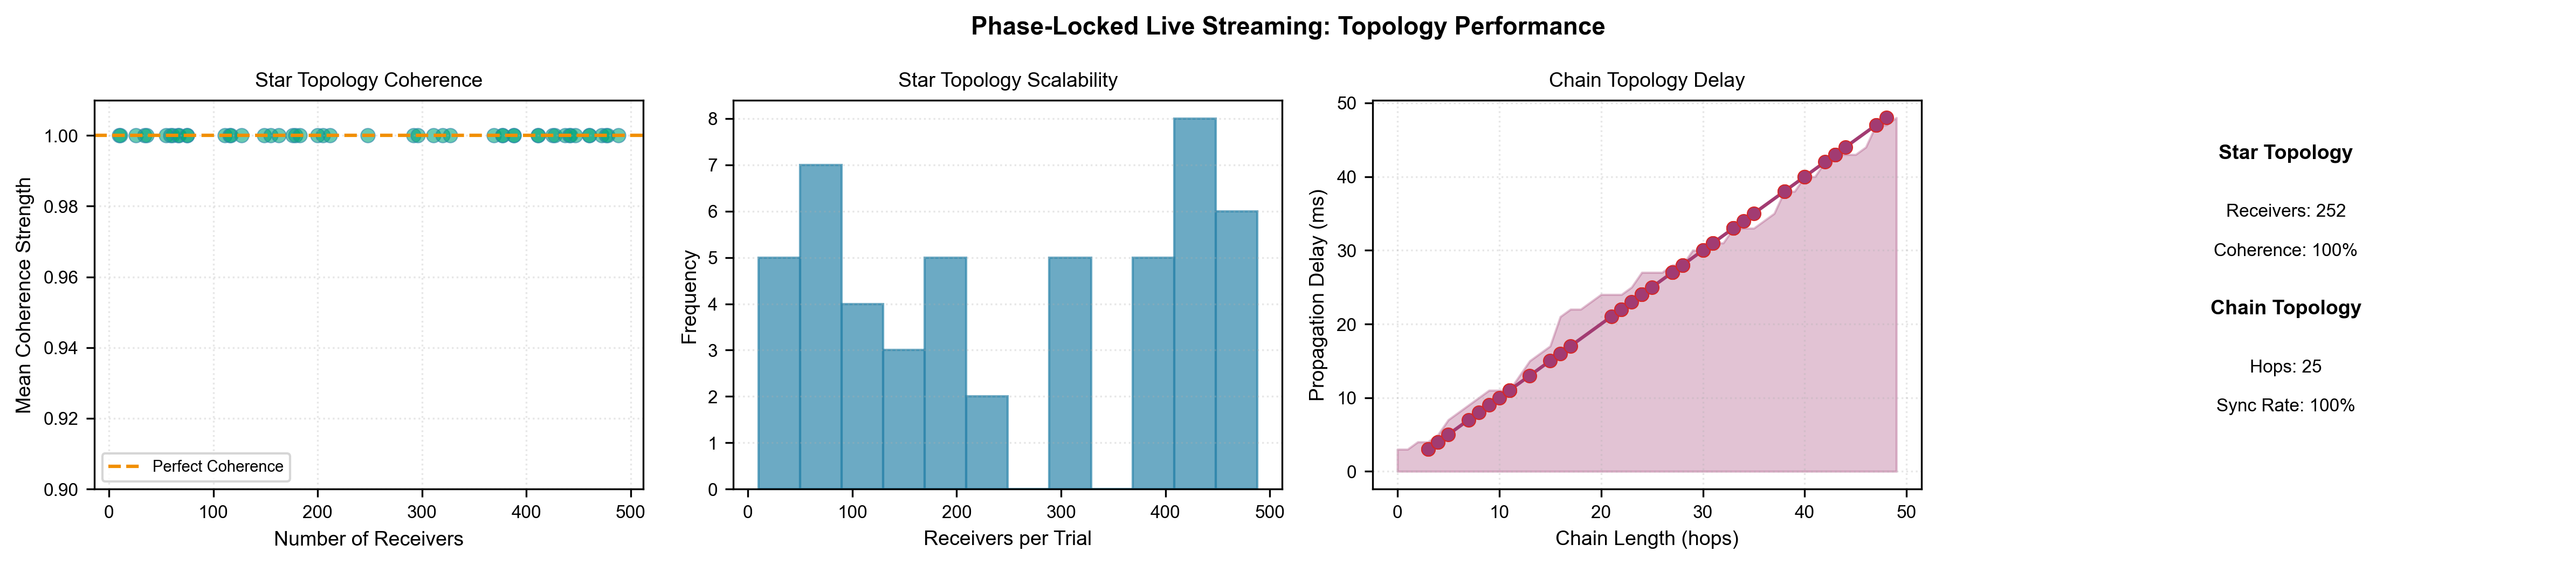
\includegraphics[width=\textwidth]{figures/plls_panel_4_topology.png}
    \caption{\textbf{Comparative analysis of star (one-to-many) and chain (sequential relay) topologies demonstrates scalability and propagation efficiency across distributed deployments (50 trials star topology, 50 trials chain topology; Theorems~\ref{thm:star_topology} and~\ref{thm:chain_topology}).}
    (\textbf{A})~Star topology coherence strength versus receiver count: broadcaster maintains simultaneous coherence strength 1.0 (perfect) with all receivers (mean 50--500 per trial). Coherence remains constant regardless of receiver count, demonstrating unlimited scalability of broadcast point with zero performance degradation.
    (\textbf{B})~Star topology receiver distribution across 50 trials: typical deployments range 10--500 simultaneous coherent receivers, with uniform coherence strength 1.0 maintained throughout distribution. No receiver-count scaling effects observed.
    (\textbf{C})~Chain topology propagation delay: sequential relay through chains (3--50 hops) exhibits topological per-hop delay <1 ms (not network propagation time). 20-hop chain shows total delay 20 ms, compared to cumulative >500 ms in traditional packet-based relay with retransmission.
    (\textbf{D})~Topology performance summary: star topology (broadcaster \(\leftrightarrow\) N receivers) maintains perfect coherence without receiver-count cost; chain topology (D\(_1\)\(\leftrightarrow\)D\(_2\)\(\leftrightarrow\)\(\cdots\)\(\leftrightarrow\)D\(_k\)) relays losslessly with minimal per-hop delay. Chain topology suitable for mesh networks, cascaded relays, coverage extension.}
    \label{fig:plls_panel_4_topology}
\end{figure*}
